% !TEX root =  ../Dissertation.tex

\chapter{Methodology}
\label{ch:methodology}

This chapter sets out the methodology used in this project in the order I implement and run it. I begin with the design
principle, which is the base that affects every later choice; namely, the portfolio ledger that runs suggested weights on any provided time frame. It is model-agnostic and is used to run every model in this project. I then download all the data, preprocess it, and set aside the holdout set. Then I train a Simple Cycle Reservoir (SCR) on the log returns and cache it for future use. I then provide these saved states to K experts and a gating network, which are linearly joined. Furthermore, the model is trained on the quality of its decisions rather than the accuracy of any forecast. That quality becomes our loss function, creating a cycle that trains our experts and the gating network. The rest of the chapter describes the statistical gates I compare against and the protocol under which I evaluate every arm. 

\section{The differentiable ledger and the decision loss}
\label{sec:ledger}

Given a weight schedule, the ledger plays the portfolio day by day and returns key metrics like Sharpe ratio, turnover, max drawdown, etc. One key point is that the weight schedule is weekly, i.e we only rebalance once per week. I do this because daily rebalances in our architecture and data would mostly chase noise, and they would also lead to extremely high net transaction costs. Returns are still calculated daily because the return values we cache are daily. The exact structure of the weight schedule is as follows

\begin{equation}
  \mathrm{targets} \in \mathbb{R}^{J \times N},
\end{equation}
where
\begin{itemize}
  \item the $J$ rows are the weekly decision points ; 
  \item the $N$ columns are the assets, the risky universe plus cash.
\end{itemize}

Each row is a target portfolio $w_t$ , thus it's important for each of its elements to be non-negative and for all elements to sum to 1. Signals are formed on the last trading day of each week and executed on the following day, so the lag between decision and execution lives outside the ledger. Transaction costs are charged on the traded notional at five basis points, cash leg included, so that turnover is paid for at every rebalance. Within a holding period the daily ledger is closed form, thus for each asset all future returns are known thus we can directly calculate for that independently of other. Since this is same for all we can use direct dot product to replace a day-by-day loop making implementation faster. Finally the ledger is written in the same tensor library as the model, so gradients flow from every daily return back to the weights that produced it making training easier. The entire data processing and portfolio ledger architecture can be visually seen in figure \ref{fig:architecture}

\begin{figure}[t]
  \centering
  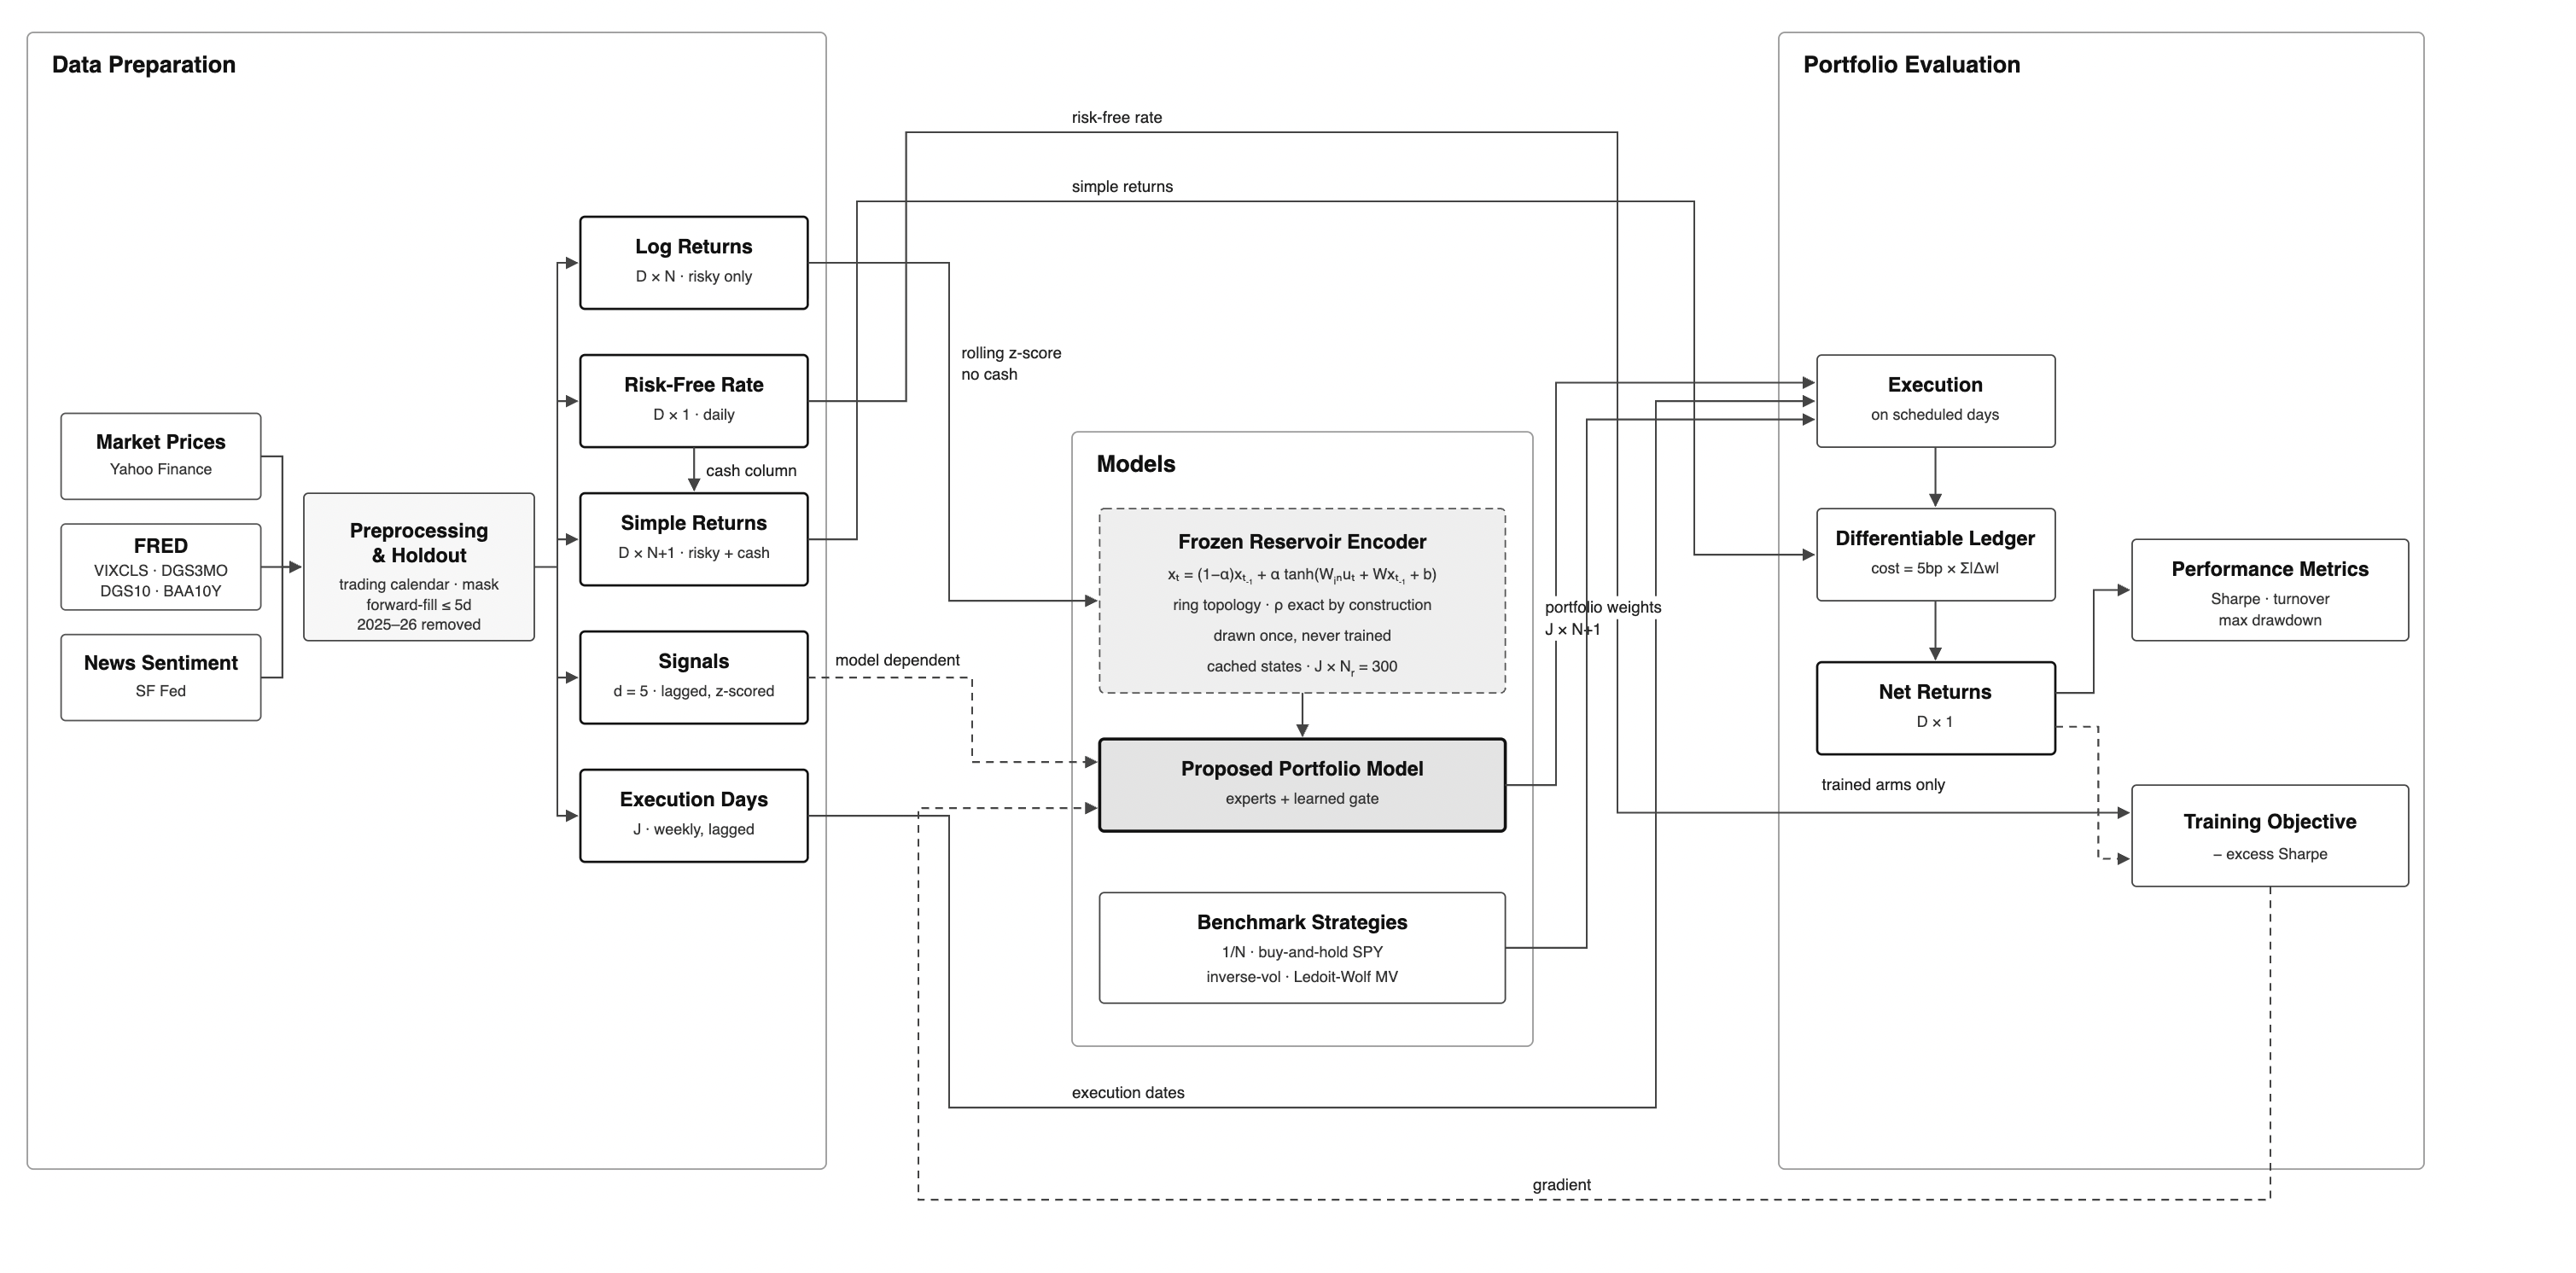
\includegraphics[width=\textwidth]{figures/arch1.png}
  \caption[System architecture]{The pipeline for input and evaluation harness. We prepare the data and daily log returns drive a frozen Simple Cycle Reservoir whose state $x_t$ is cached once. Any model can produce a
  portfolio which is played through a differentiable ledger with transaction costs, and its excess Sharpe ratio defines the loss.}
  \label{fig:architecture}
\end{figure}

Let $r^{\text{net}}_{t}$ denote the daily net return of the blended portfolio and $r^{f}_{t}$ the risk-free rate that cash earns over the same day. The primary training signal is the annualised excess Sharpe ratio of the realised stream,
\begin{equation}
  \operatorname{SR} = \sqrt{252}\;
  \frac{\operatorname{mean}_t\big(r^{\text{net}}_{t} - r^{f}_{t}\big)}
       {\sqrt{\operatorname{var}_t\big(r^{\text{net}}_{t} - r^{f}_{t}\big)} + \varepsilon},
  \label{eq:sharpe}
\end{equation}
with a small constant $\varepsilon$ that keeps the ratio finite when the excess stream is near zero. This is needed for cash, where both the numerator and denominator would be zero, or, in practice, an arbitrarily small number, which would give an unpredictable Sharpe; adding this makes its Sharpe 0, so it does not accidentally become a money haven. For our project, I set it to $10^{-6}$. The same $\varepsilon$ appears in the reporting metric, so the quantity optimized is the quantity reported. The training loss is the negative Sharpe ratio with two optional penalties,
\begin{equation}
  \mathcal{L} = -\operatorname{SR}
     + \lambda_{\text{cvar}}\,\operatorname{CVaR}_{95}
     + \lambda_{\text{bal}}\,\operatorname{CV}^2
  \label{eq:loss}
\end{equation}
where the first penalty is meant to prevent the worst outcomes(i.e. days with huge loss) through the conditional value-at-risk of the excess stream and the second discourages expert collapse using square of coefficient of variation(CV). This is calculated as follows:

\begin{equation}
  \mathrm{CV}^2(I) = \frac{\sigma_I^2}{\bar{I}^{\,2}},
  \qquad
  \bar{I} = \frac{1}{K}\sum_{k=1}^{K} I_k,
  \qquad
  \sigma_I^2 = \frac{1}{K}\sum_{k=1}^{K}\big(I_k - \bar{I}\big)^2,
\end{equation}
where $I_k = \dfrac{1}{T}\sum_{t=1}^{T}\pi_{t,k}$ is the mean weight of that expert gate over the $T$ decisions. The load-balancing term is identically zero at $K = 1$. Both weights are searchable and default to zero, so the plain objective is $-\operatorname{SR}$.
The Sharpe ratio couples every day,i.e its value can be calculated on any number of days, and its value on all days in the fold is the value we optimize on rather than on mini-batches.

\section{The frozen reservoir}
\label{sec:reservoir}

At the core of our project is a frozen Simple Cycle Reservoir. This is a  fixed and deterministic recurrent system driven by the input log returns, from which only a lightweight readout is trained. The central driving equation to obtain the states of the reservoir is as follows:
\begin{equation}
  x_t = (1-\alpha)\, x_{t-1} + \alpha \tanh\!\big(W x_{t-1} + v\, W_{\text{in}} u_t\big),
  \label{eq:reservoir}
\end{equation}
where 

\begin{equation}
  u_t \;=\;
  \begin{pmatrix} r_{1,t} \\ r_{2,t} \\ \vdots \\ r_{M,t} \end{pmatrix}
  \;=\;
  \begin{pmatrix}
    \ln\!\big(P_{1,t}/P_{1,t-1}\big) \\[2pt]
    \ln\!\big(P_{2,t}/P_{2,t-1}\big) \\[2pt]
    \vdots \\[2pt]
    \ln\!\big(P_{M,t}/P_{M,t-1}\big)
  \end{pmatrix}
  \;\in\; \mathbb{R}^{M}.
  \label{eq:reservoir-input}
\end{equation}

\begin{itemize}
  \item $x_t \in \mathbb{R}^{N}$ is the reservoir state at time t;
  \item $\alpha \in (0,1]$ is the leak rate (smaller $\alpha$ $\Rightarrow$ longer memory);
  \item $W \in \mathbb{R}^{N\times N}$ is the fixed recurrent matrix (the Simple Cycle ring);
  \item $W_{\mathrm{in}} \in \mathbb{R}^{N\times M}$ is the fixed input matrix;
  \item $P_{i,j}$ is the adjusted closing price of asset $i$ on day $t$
\end{itemize}

Here we have two matrix, both matrices follow the Simple Cycle Reservoir construction given in Section~\ref{sec:bg-scr-construction} exactly (Eqs.~\ref{eq:scr-recurrent}--\ref{eq:scr-input-vdc}); nothing in them is trained or drawn at random.

Three implementation choices matter for later chapters. First, the input scale $v$ is not set by hand but calibrated so that the standard deviation of the pre-activation $W x_{t-1} + v W_{\text{in}} u_t$ reaches a target of about $0.7$, which places the activations in the curved part of $\tanh$ without saturating them; the calibration uses only the first $60\%$ of the sample and so never sees the evaluation period. Second, the first $250$ trading days of each driven series are discarded as a washout, so the arbitrary choice $x_0 = 0$ has decayed away before any state is used. Third, because the reservoir is never trained, its states can be computed once over the whole sample and cached; a training run then reads precomputed states instead of driving the recurrence, which is what makes the roughly one thousand fits in the study affordable on a laptop.



\section{The regime gate and the expert mixture}
\label{sec:gate}

\begin{figure}[t]
  \centering
  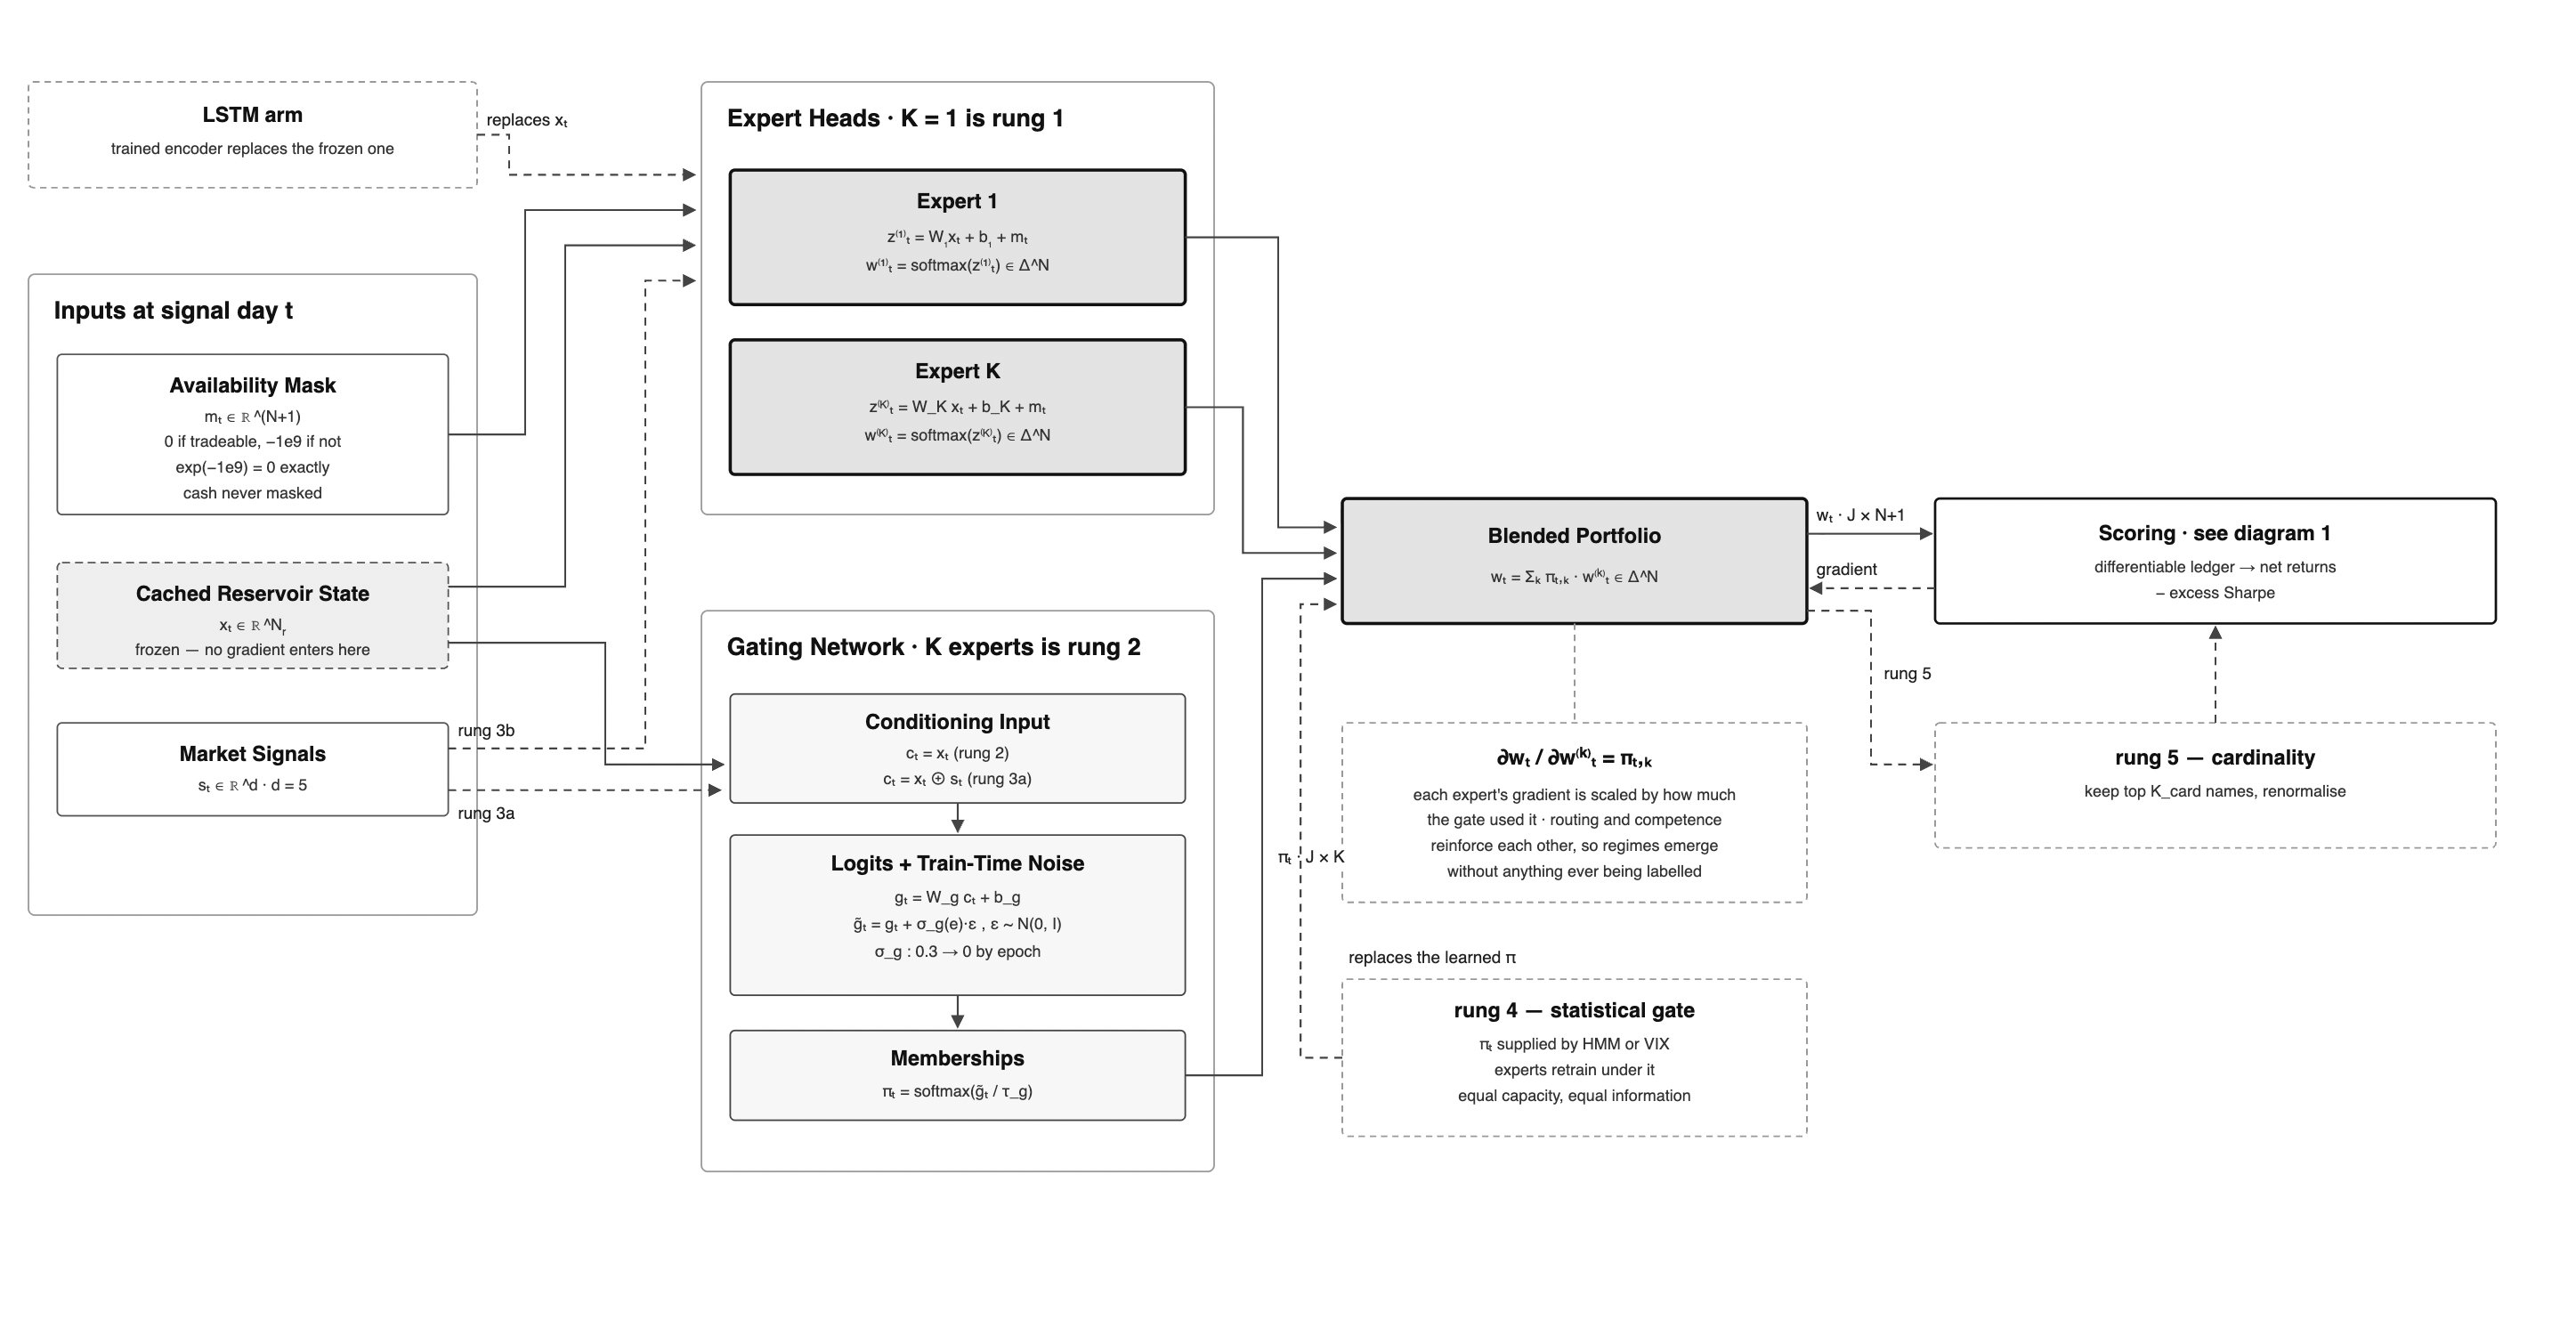
\includegraphics[width=\textwidth]{figures/arch2.png}
  \caption[Model architecture]{The reservoir inputs (and optionally market sentiment) are provided both of gates and experts and are combined together to generate final model's portfolio suggestion.}
  \label{fig:arch2}
\end{figure}

The trained part of the model is a mixture of experts \cite{jacobs1991adaptive}. At each weekly decision day $t$ the reservoir supplies the state $x_t$, and two kinds of readout act on it. The first is the experts, they are defined as follows

\begin{equation}
  w_t^{(k)} = \operatorname{softmax}\!\big(W_k x_t + m_t\big),
  \label{eq:expert}
\end{equation}
in which $m_t$ is an additive mask whose entries are $0$ for assets that are tradeable on day $t$ and a large negative constant otherwise, so that the softmax weight on an unavailable asset underflows to exactly zero while cash is never masked. This is required because two assets in the sector universe were added long after its inception.

The second is the gating network that produces a softmax response where the values are how likely the gating network believe the corresponding expert to be.
\begin{equation}
  \pi_t = \operatorname{softmax}\!\Big( \big(W_g x_t + b_g + \sigma_g\,\varepsilon_t\big)/\tau \Big),
  \qquad \varepsilon_t \sim \mathcal{N}(0, I_K),
  \label{eq:gate}
\end{equation}
where $W_g x_t + b_g$ are the gate logits, $\tau$ is the temperature that controls
how sharply the membership concentrates, and $\sigma_g\,\varepsilon_t$ is Gaussian
exploration noise added to the logits \emph{during training only}
($\sigma_g = 0$ at evaluation). The noise standard deviation is annealed linearly
to zero,
\begin{equation}
  \sigma_g(e) = \sigma_0 \,\max\!\Big(0,\; 1 - \frac{e}{P}\Big),
  \qquad \sigma_0 = 0.3, \quad P = 2\,\text{patience},
  \label{eq:gate-noise}
\end{equation}
so the routing explores early before the experts have differentiated, so no
expert is starved and the gate commits once the noise has decayed to zero at
epoch $P$.

The final target portfolio is the membership-weighted blend of the experts,
\begin{equation}
  w_t = \sum_{k=1}^{K} \pi_{t,k}\, w_t^{(k)}.
  \label{eq:blend}
\end{equation}

The number of experts $K$ is a configuration parameter rather than a fixed
constant. At $K = 1$ the mixture reduces provably to a single trained head and
the gate is inert, which gives a clean baseline within the same code. Market-level signals may optionally be concatenated to the state before the gate, the experts, or both; keeping the signals market-level, and separate from the per-asset state, is what lets us treat them as an input the gate \emph{may} use rather than as a definition of a regime. This entire architecture can be seen visually at \ref{fig:arch2}.

\section{Design principle: decision-focused learning}
\label{sec:principle}

A conventional pipeline forecasts each asset's return and then hands those forecasts to a separate optimiser. The forecaster is trained to minimise a prediction error such as the mean squared error, which is a proxy for the thing we actually care about. The proxy and the objective can disagree. A model with the lower prediction error can still make the worse allocation. Methods like minimizing MSE treats every asset's error as equally important and symmetric. But for the allocation, an error in a high-weight asset matters far more than in a near-zero-weight one, An overconfident forecast that preserves the correct ranking is harmless to the decision. Training on the surrogate optimises the wrong quantity whenever the two come apart, and they come apart precisely because the model is imperfect \cite{elmachtoub2022smart}. To understand this fully consider the following example  Two assets, $A$ and $B$, will realise returns of $4\%$ and $1\%$ respectively. Two models forecast these returns, and a simple strategy acts on each forecast by buying the single asset it rates highest; the strategy then earns that asset's \emph{actual} return. Table~\ref{tab:mse-vs-decision} shows the outcome.

\begin{table}[h]
  \centering
  \begin{tabular}{lccccc}
    \hline
             & Asset $A$ & Asset $B$ & MSE & buys & earns \\
    \hline
    Actual   & $4\%$ & $1\%$   & ---  & ---   & ---   \\
    Model 1  & $2\%$ & $3\%$   & $4.0$ & $B$   & $1\%$ \\
    Model 2  & $7\%$ & $-1\%$  & $6.5$ & $A$   & $4\%$ \\
    \hline
  \end{tabular}
  \caption{A more accurate forecast can make the worse decision. Model~1 has the lower mean squared error but earns less, because its small errors flip the ranking of the two assets, while Model~2's larger error preserves it.}
  \label{tab:mse-vs-decision}
\end{table}

The mean squared errors are
\begin{equation}
  \mathrm{MSE}_1 = \tfrac{1}{2}\big[(2-4)^2 + (3-1)^2\big] = 4.0,
  \qquad
  \mathrm{MSE}_2 = \tfrac{1}{2}\big[(7-4)^2 + (-1-1)^2\big] = 6.5,
\end{equation}
so by prediction error Model~1 is the better forecaster ($4.0 < 6.5$). Yet it is the worse investor: it rates $B$ above $A$ and earns $1\%$, whereas Model~2 rates $A$ above $B$ and earns $4\%$.

I therefore train end to end on the decision itself. The loss is the risk-adjusted quality of the entire realised return stream, measured by the excess Sharpe ratio \cite{sharpe1994sharpe}, and the gradient of that loss flows back through the portfolio and into the parameters that produced it. No part of the system forecasts a return. This choice is what makes the accounting ledger of Section~\ref{sec:ledger} a differentiable object rather than a reporting step: the ledger \emph{is} the forward pass of the loss. Additionally since we are optimizing Sharpe ratio this also accounts for volatility as well instead of just profits.

The same principle motivates the research question the study is built to answer. If regimes are useful, they should be discovered by the decision objective, not imposed beforehand by a statistical rule. The falsifiable question is whether decision-defined regimes carve the market differently from, and outperform, statistically defined regimes at equal capacity and equal information. Sections~\ref{sec:gate} and~\ref{sec:baselines} construct the two sides of that comparison so that they differ only in how the regimes are formed.

\begin{algorithm}[t]
  \caption{Decision-focused training of one mixture on one fold}
  \label{alg:train}
  \begin{algorithmic}[1]
    \STATE \textbf{input:} cached states $x$, train/validation packs, experts $K$, loss weights, seed
    \STATE initialise gate $\{W_g,b_g\}$ and experts $\{H_k\}$ from the seed
    \STATE $\text{best} \gets -\infty$
    \FOR{epoch $= 1,2,\dots$ until early stopping}
      \STATE $\pi_t \gets$ gate$(x_t)$ with annealed logit noise \COMMENT{Eq.~\ref{eq:gate}}
      \STATE $w_t \gets \sum_k \pi_{t,k}\, w_t^{(k)}$ over the training fold \COMMENT{Eq.~\ref{eq:blend}}
      \STATE run the differentiable ledger to obtain $r^{\text{net}}_{t}$
      \STATE $\mathcal{L} \gets -\operatorname{SR} + \lambda_{\text{cvar}}\operatorname{CVaR}_{95} + \lambda_{\text{bal}}\operatorname{CV}^2$ \COMMENT{Eq.~\ref{eq:loss}}
      \STATE backpropagate $\mathcal{L}$ and update the gate and experts only
      \STATE evaluate the noise-free Sharpe on the validation fold
      \IF{validation Sharpe improves}
        \STATE $\text{best} \gets$ current parameters
      \ENDIF
    \ENDFOR
    \RETURN the parameters at \text{best}
  \end{algorithmic}
\end{algorithm}


\section{Naive baselines and Statistical gates}
\label{sec:baselines}

\paragraph{Naive baselines:}
Four allocation rules with no regime structure set the humility line: an equal-weight portfolio over the active universe, an inverse-volatility portfolio on a $63$-day window, buy-and-hold on the market index, and a Ledoit-Wolf shrinkage mean-variance portfolio \cite{ledoit2004honey} that holds risky assets under a budget constraint and leaves the residual in cash. Every baseline is run through the same ledger, the same cost model and the same evaluation windows as the learned arms.

\paragraph{Filtered hidden Markov gate:}
A Gaussian hidden Markov model \cite{hamilton1989new,rabiner1989tutorial} is fitted, on the training window only, to two market observables: the equal-weight excess return of the active universe and its trailing $21$-day realised volatility. Each hidden state $k$ emits observations from a diagonal Gaussian $\mathcal{N}(\mu_k,\Sigma_k)$, and a transition matrix $A$ governs how states follow one another. The membership used at day $t$ is the \emph{filtered} posterior $p(\text{state}_t \mid o_{1:t})$, computed by a forward recursion in log space,

\begin{equation}
  \log \alpha_t(j) = \operatorname{logsumexp}_i\big(\log \alpha_{t-1}(i) + \log A_{ij}\big)
      + \log \mathcal{N}(o_t;\,\mu_j,\Sigma_j),
  \qquad \pi_t = \frac{\alpha_t}{\textstyle\sum_j \alpha_t(j)}.
  \label{eq:forward}
\end{equation}
The forward filter conditions only on observations up to and including day $t$. The library routine returns \emph{smoothed} posteriors from the forward-backward algorithm, which condition on the whole sequence, future included, and would have handed the baseline information the learned system never has.

\paragraph{VIX-tercile gate:}
The simpler statistical gate classes each day by where the previous day's VIX level sits against the terciles of its own trailing year. A one-hot membership over low, mid, and high. The level itself is lagged one day and the tercile boundaries are lagged one day beyond the window that formed them, so a value is never compared against a window that contains it.

\paragraph{Gate Analysis:}
To understand the underlying significant factors of the gates we need a single number, comparable across schemes, saying how much of a given market variable a labelling accounts for. Each weekly decision day $t$ carries a regime label $k_t \in \{1,\dots,K\}$ from one scheme and a value $v_t$ of one market variable, like trailing realised volatility or the five-day return. We can treat the $K$ regimes as groups, the total variance $v$ will split into a part explained by the labeling and a part left to the regime, and $\eta^2$ is key quantifying metric,

\begin{equation}
  \eta^2 \;=\; \frac{\mathrm{SS}_{\text{between}}}{\mathrm{SS}_{\text{total}}}
  \;=\;
  \frac{\sum_{k=1}^{K} n_k \big(\bar{v}_k - \bar{v}\big)^2}
       {\sum_{t=1}^{T} \big(v_t - \bar{v}\big)^2},
  \label{eq:eta2}
\end{equation}
where $n_k$ is the number of weeks in regime $k$, $\bar{v}_k$ the mean of $v$ over those weeks, and $\bar{v}$ the mean over all $T$ weeks. It is bounded in $[0,1]$: at $0$ the regimes are uninformative about $v$, since every regime has the same mean. At $1$ the labelling separates $v$ perfectly. Reading $\eta^2$ down a column of variables therefore says what a scheme is tracking, and reading across schemes says whether two of them track the same thing. 

\section{Evaluation protocol}
\label{sec:evaluation}

\paragraph{Walk-forward folds:}
Models are evaluated on a rolling walk-forward, illustrated in Figure~\ref{fig:walkforward}. Each fold trains on all data up to a point, uses the following calendar year for validation and early stopping, and reports on the year after that. A short portion is removed from the tail of each training window so that nothing with memory crosses the train-validation boundary. Adjacent folds share a year, since the test year of one fold is the validation year of the next. I quantify that overlap rather than hide it. Also each evaluated year starts from cash for both models and baselines.

\paragraph{Aggregation:}
Per-fold Sharpe ratios are not simply averaged. The Sharpe ratio is a non-linear statistic, and averaging it across years will account for wealth each January and weights a calm year equally with a crisis year. Instead each seed's fold segments are stitched into one continuous daily stream and scored once, which is exactly how a baseline running continuously would be scored. Per-year figures are reported beside the headline as a consistency breakdown, never as the headline itself. Reported Sharpe ratios annualise with $\sqrt{252}$ for comparability with the literature.

\begin{figure}[t]
  \centering
  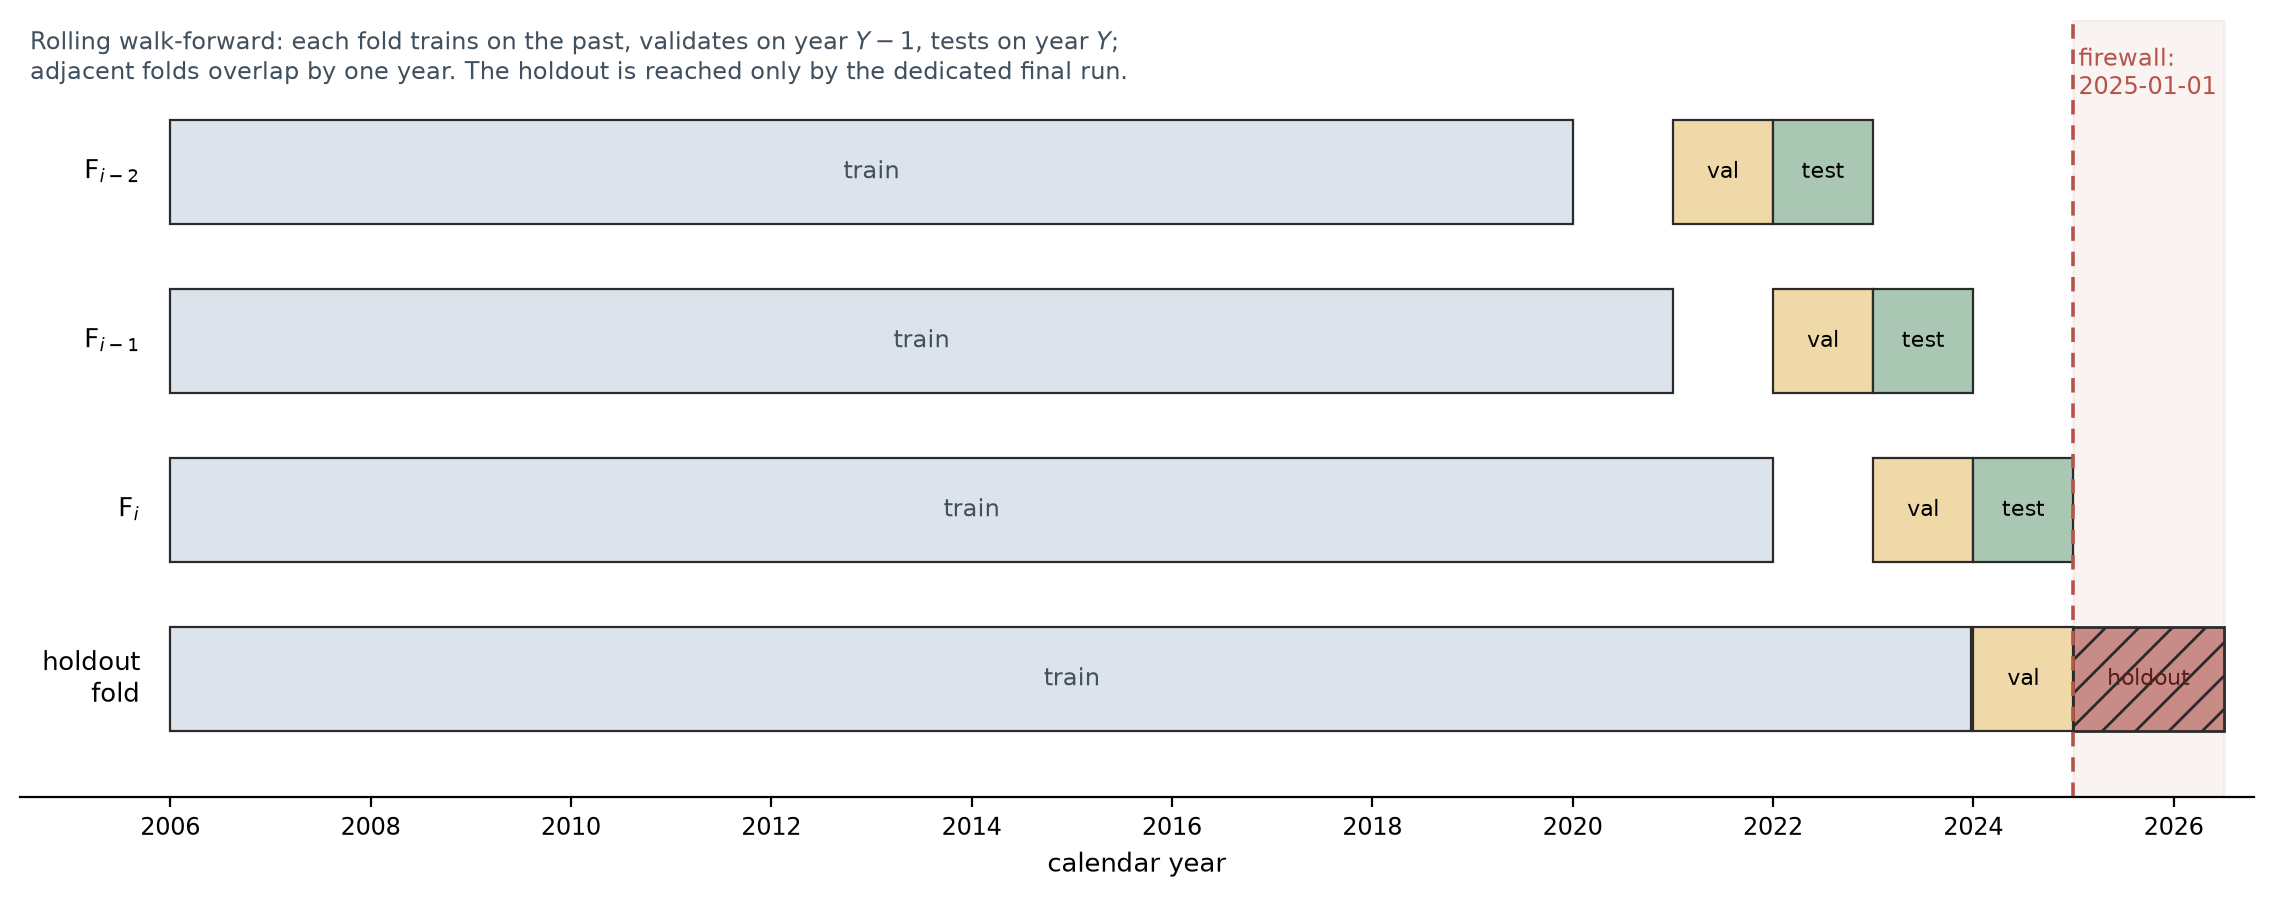
\includegraphics[width=\textwidth]{fig_walkforward.png}
  \caption[Walk-forward and holdout protocol]{The rolling walk-forward. Each fold trains on the past, validates on year $Y-1$ and tests on year $Y$; adjacent folds overlap by one year. The final period is firewalled as a holdout, it is removed from every artifact at load time and reached only once, by a dedicated final run.}
  \label{fig:walkforward}
\end{figure}

\paragraph{The holdout:}
A final block of data is held out and firewalled in code. It is removed from every artifact as it is loaded, so those dates are absent from memory in every run rather than merely unevaluated, and a guard raises an error if any evaluation window crosses the boundary. The holdout is touched exactly once, by a dedicated run, after the configuration has been frozen, and its result is reported against the trial count as it stands at that moment. It is expected to carry little statistical weight, being a single short path, but high credibility, since nothing about the configuration can have been chosen with knowledge of it.
